\section{Sources}
\label{sec:sources}

The mapping can be deduced based on the following information:
\begin{itemize}
  \item geometric information from ICARUS detector blueprints~\cite{SBNDocDB1020}
    (with the caveat that second induction and collection planes on one of the
    TPCs are swapped, see \cref{fig:WirePlanesInTPC})
  \item undocumented information on the cabling, reported in \cref{ssec:CablingInfo}
  \item information from the (currently unpublished) general technical note
    on the TPC connectivity test~\cite{SBNDocDBxxxx:ConnTest},
    replicated in \cref{ssec:PlaneAssignment}
\end{itemize}


\subsection{Cabling details}
\label{ssec:CablingInfo}

This information was provided by Angela Fava:
\begin{itemize}
  \item all cables are installed sequentially at the TPC end, and the wires within the flat cable are numbered following the same sequence;
  \item for Induction1 A1-33, B1-33, C1-33 and D-133 are all top to bottom (therefore the red conductor is at the top);
  \item for corners F1-17 and H1-17 are bottom to top, while E1-17 and K1-17 are top to bottom;
  \item please note that there is a mistake in Fig. 2 at page 7 in the tech note, in that the South-East corner is Collection and the North-East is Induction 2;
  \item for standard chimneys 1 to 9 and 10 to 18 SHOULD be North to South, but for cross-checking this I have asked photo documentation to Andrea Zani and Claudio and I am waiting on their reply.
\end{itemize}


\subsection{Assignment of wire planes to minicrate sides}
\label{ssec:PlaneAssignment}

\begin{figure}[p]
  \centerline{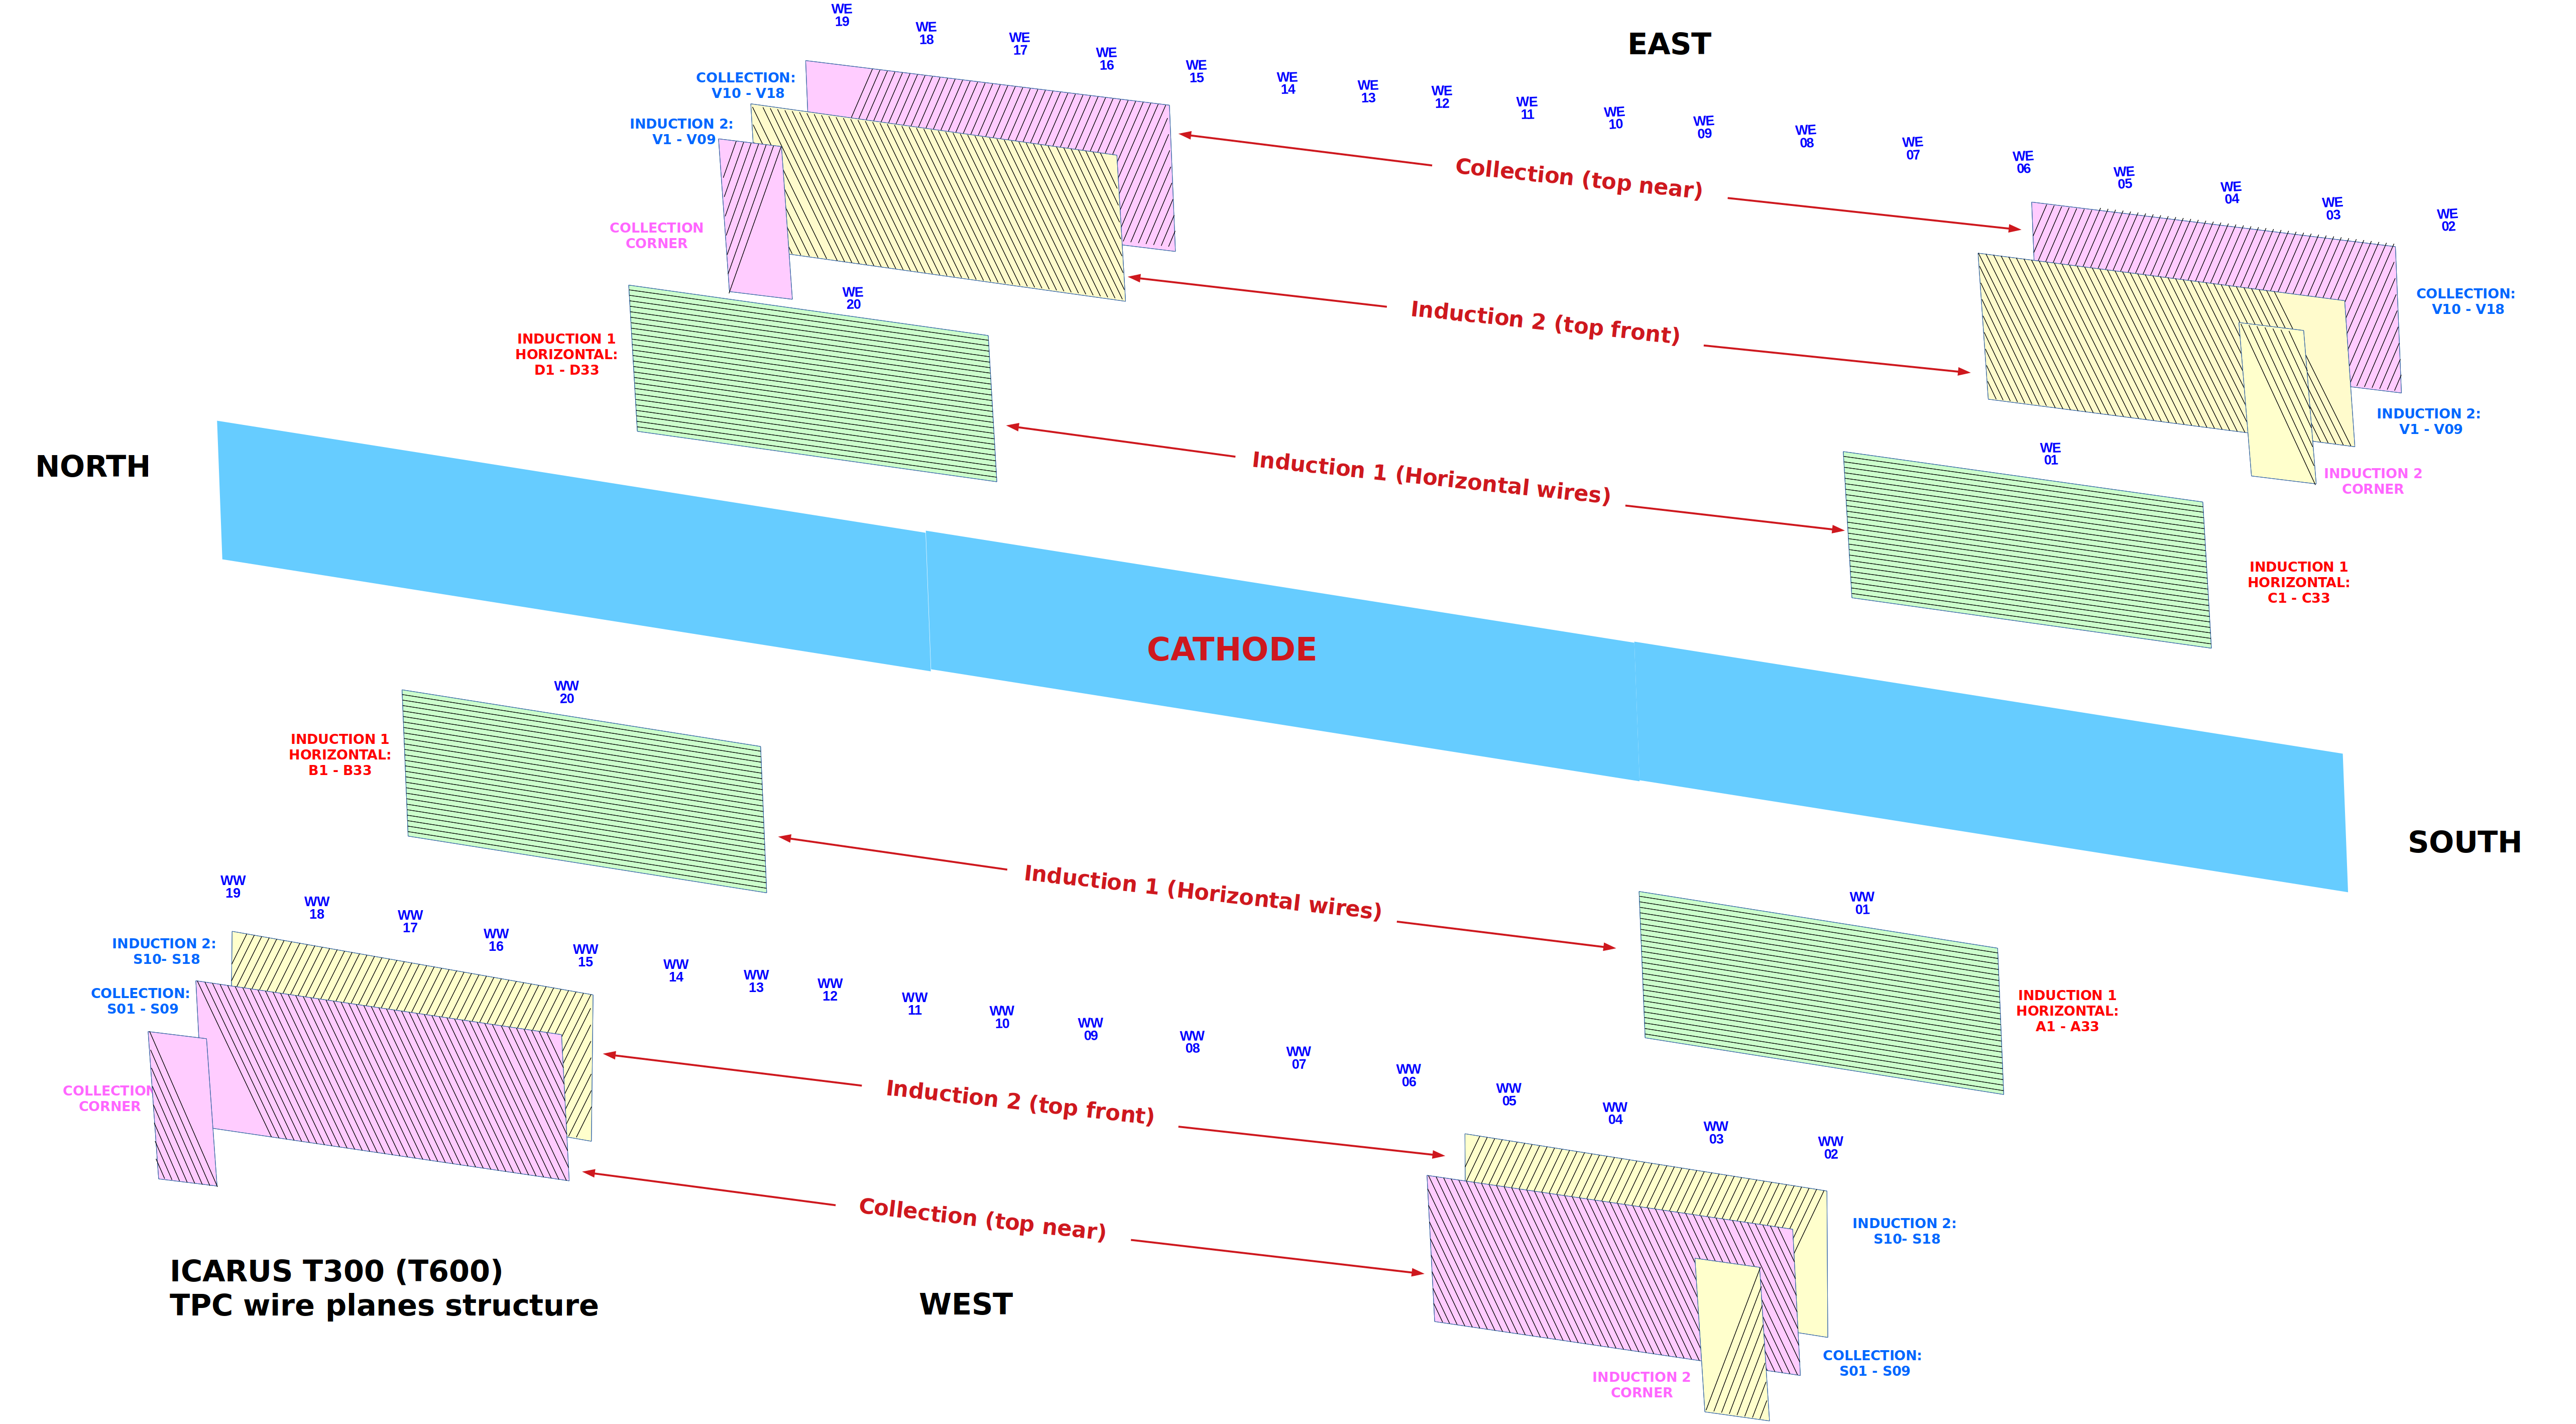
\includegraphics[width=0.8\textheight,angle=90]{figures/Icarus_TPC_wp}}
  \caption{
    Wire planes in a cryostat and their disposition (from~\cite{SBNDocDBxxxx:ConnTest}).
    Note the orientation of the wires, correct and contrasting with the erroneous one in~\cite{SBNDocDB1020}.
    \label{fig:WirePlanesInTPC}
  }
\end{figure}

This information is extracted from a technical note~\cite{SBNDocDBxxxx:ConnTest} describing the TPC connectivity test:
\begin{itemize}
  \item in chimneys WW and EW:
    \begin{itemize}
      \item flat cables from 1 to 9 are connected to wires on the \emph{collection plane}
      \item flat cables from 10 to 18 are connected to wires on the \emph{second induction plane}
    \end{itemize}
  \item in chimneys WE and EE:
    \begin{itemize}
      \item flat cables from 1 to 9 are connected to wires on the \emph{second induction plane}
      \item flat cables from 10 to 18 are connected to wires on the \emph{collection plane}
    \end{itemize}
\end{itemize}


